\label{acc_simulations}
\indent


\clearpage

\subsubsection{Acceptance simulations for J/$\Psi$}
\indent

The generator used for J/$\Psi$ acceptance studies simulates multi-particle final states in photo- and electro production reactions. It has correct decay channels and branching ratios for most of particles listed in PDG (Lund/Jetset \cite{lepto}) and allows to set the kinematic dependencies, e.g. Q$^2$ and $t$. The reaction: 
\begin{eqnarray}
ep\to e^\prime~J/\Psi~p^\prime\to e^\prime\mu^+\mu^-p^\prime
\end{eqnarray}
was simulated with the following conditions:
\begin{itemize}
\item beam energy $E=11$ GeV
\item electron four momentum transferred dependence $1/{Q^4}$ ($Q^2=-q^2=-(k_i-k_f)^2$, where $k_{i(f)}$ is the initial (final) four momentum of the electron)
\item exponential dependence for the squared four-momentum transfer from initial to final state proton, $e^{3t}$, ($t=(p_i-p_f)^2$, where $p_i$ and $p_f$ are four momenta of the initial and final state protons)
\end{itemize}

The Q$^2$- and t-dependences as they have been generated initially and their form after the electron is selected in the calorimeter detection range are shown in Fig.\ref{fig:jp_sim}. The cutoff on maximum Q$^2$ and t after electron selection are due to the minimum momentum, $p_{min}=0.5$ GeV, and the maximum angel, $\theta_{max}=35^\circ$ limits.

\begin{figure}[htbp]
\begin{center}
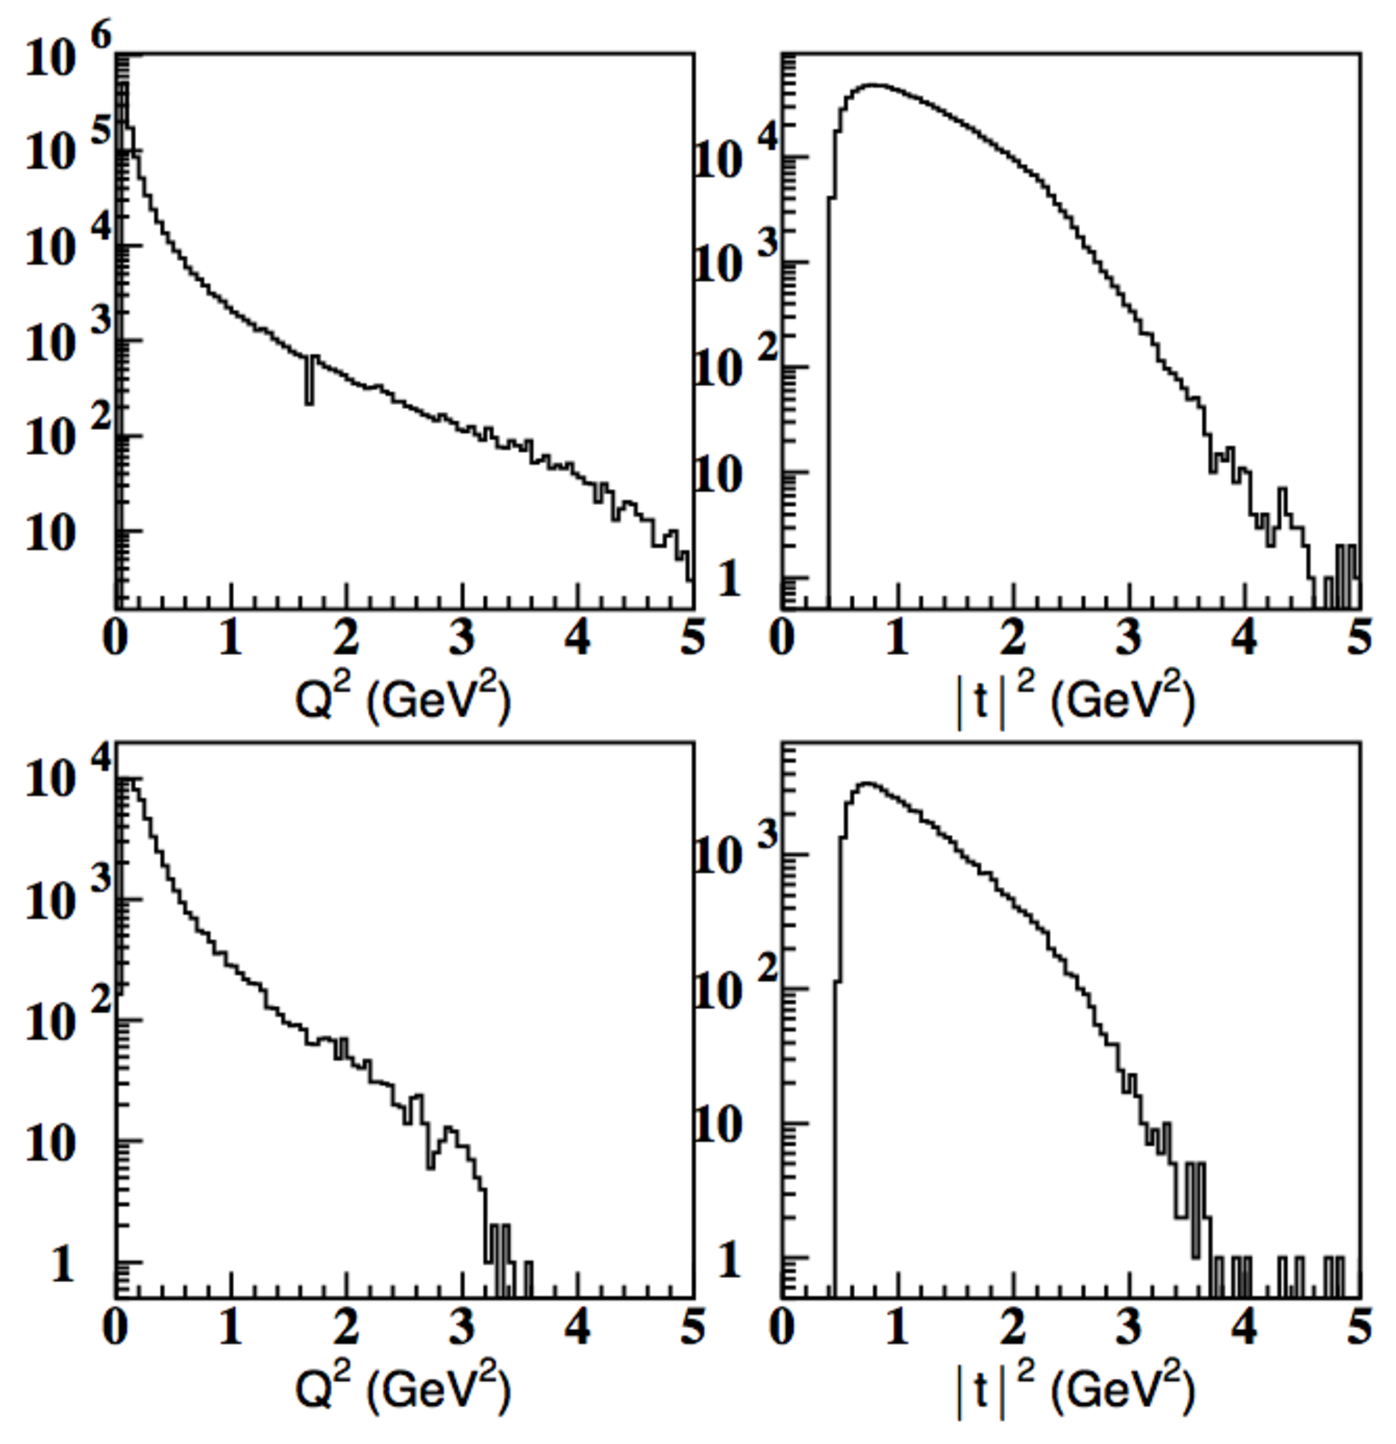
\includegraphics[width=0.8\textwidth]{jpsi_q2_t_sim.pdf}
\caption{Simulated Q$^2$ and $t$ distributions, top. On the bottom panels the same distributions when electron is detected in the calorimeter.  }
\label{fig:jp_sim}
\end{center}
\end{figure}

In Fig.\ref{fig:jp_kine}, momentum vs. scattering angle distributions for final state particles in the reaction $ep\to e^\prime p^\prime J/\Psi$ are shown. Due to large momentum transfer, near threshold  production, recoil protons will scatter at forward direction and will not be detected. Electrons will be detected in the calorimeter as was described above in the angular rage $5^\circ < \theta_e <35^\circ$ with momentum $p>0.5$ GeV/c. The muons are produced mostly in forward angles ($\theta_\mu<40^\circ$), bottom left panel of Fig.\ref{fig:jp_kine}, and remain in the same momentum-angular space with electrons in the calorimeter, bottom right panel. The CLAS12 FD that can detect changed tracks in angular range $5^\circ < \theta <35^\circ$ is well suited for detecting muons from presented reaction. In Fig.\ref{fig:jp_mukine} momentum vs scattering angle of $\mu^+$ and $\mu^-$ are shown. Due to large momentum there is not much difference in detection acceptance for negatively and positively charged tracks at forward angles due to the magnetic field and the CLAS12 detector acceptances.

\begin{figure}[htbp]
\begin{center}
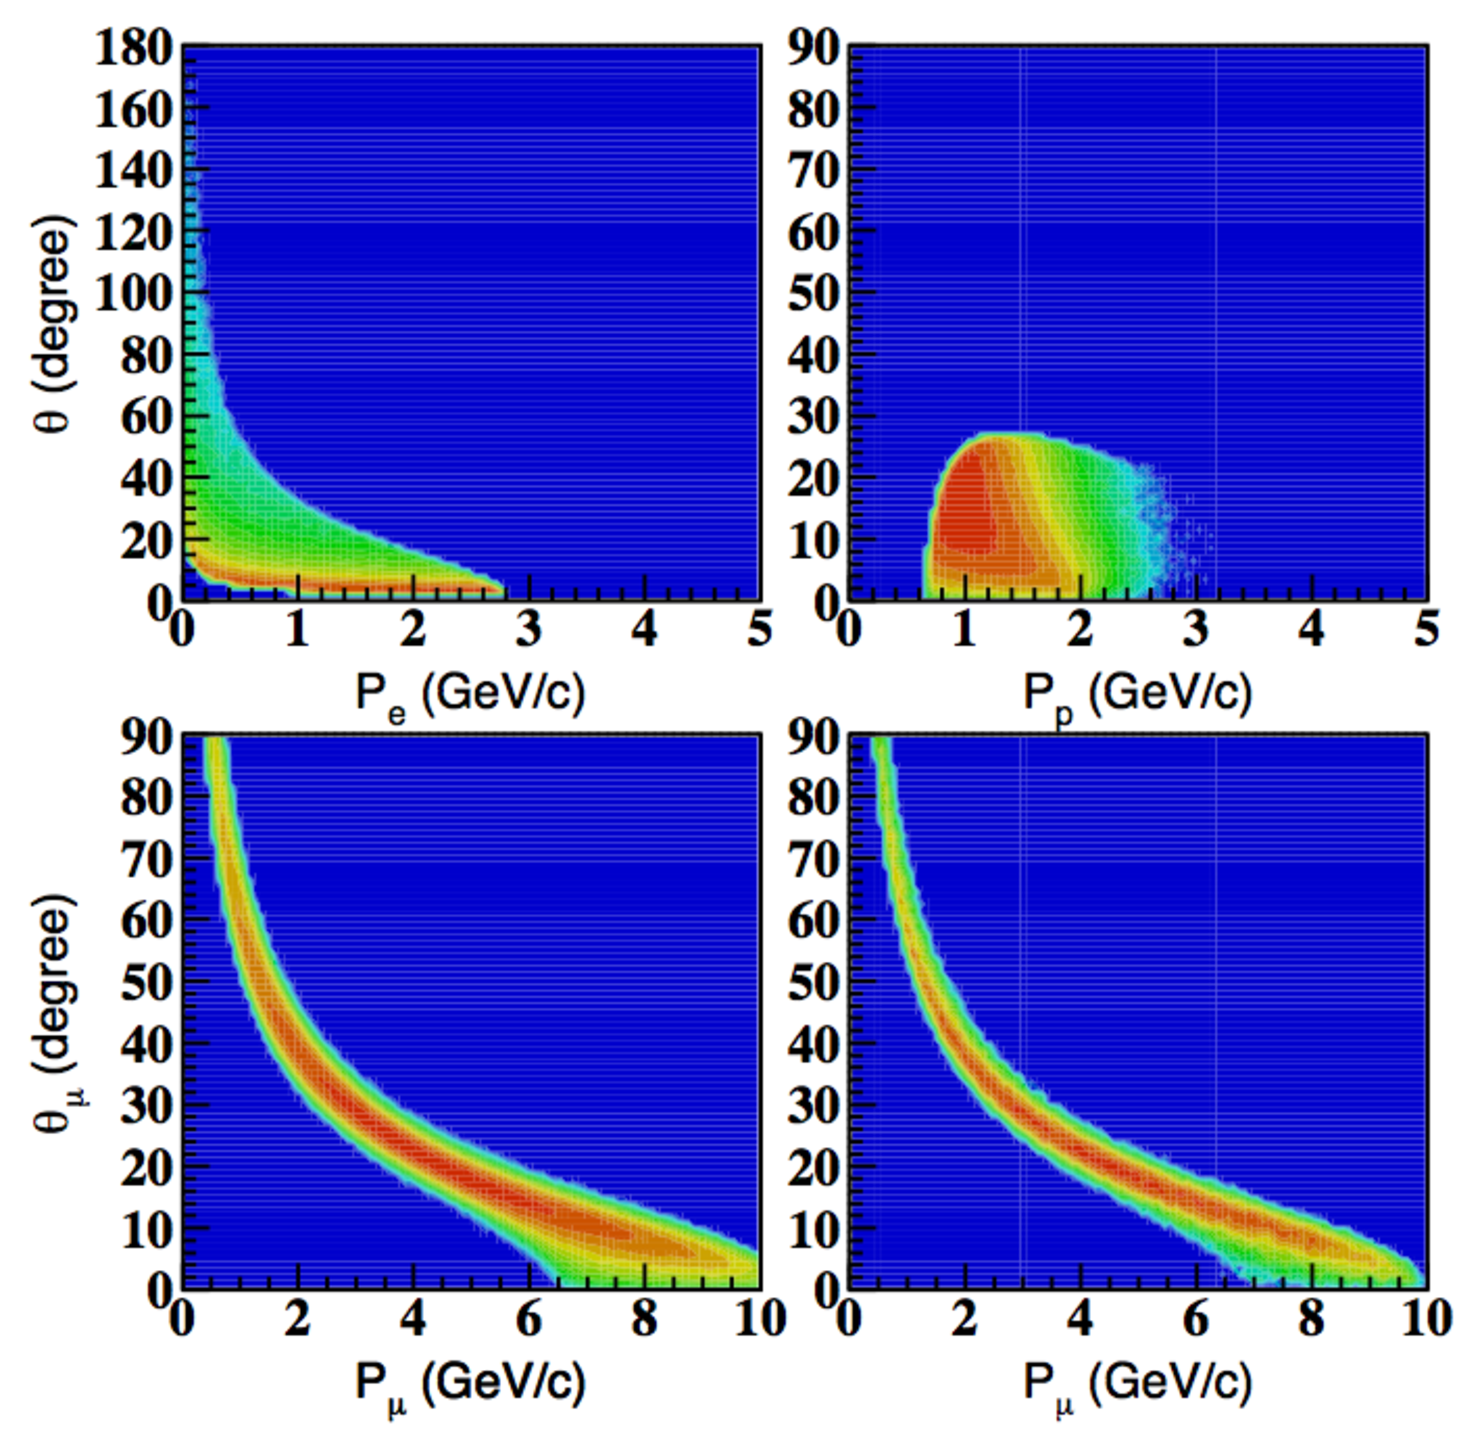
\includegraphics[width=0.8\textwidth]{jpsi_kine.pdf}
\caption{Kinematics of the scattered electron, recoil proton, and the decay muons for the reaction $ep\to e^\prime p^\prime J/\Psi $. In the bottom-right panel angular-momentum distribution of muons is shown for events where electron momentum is $p>0.5$ GeV and is in the scattering angular range $5^\circ <\theta<35^\circ$.}
\label{fig:jp_kine}
\end{center}
\end{figure}

\begin{figure}[htbp]
\begin{center}
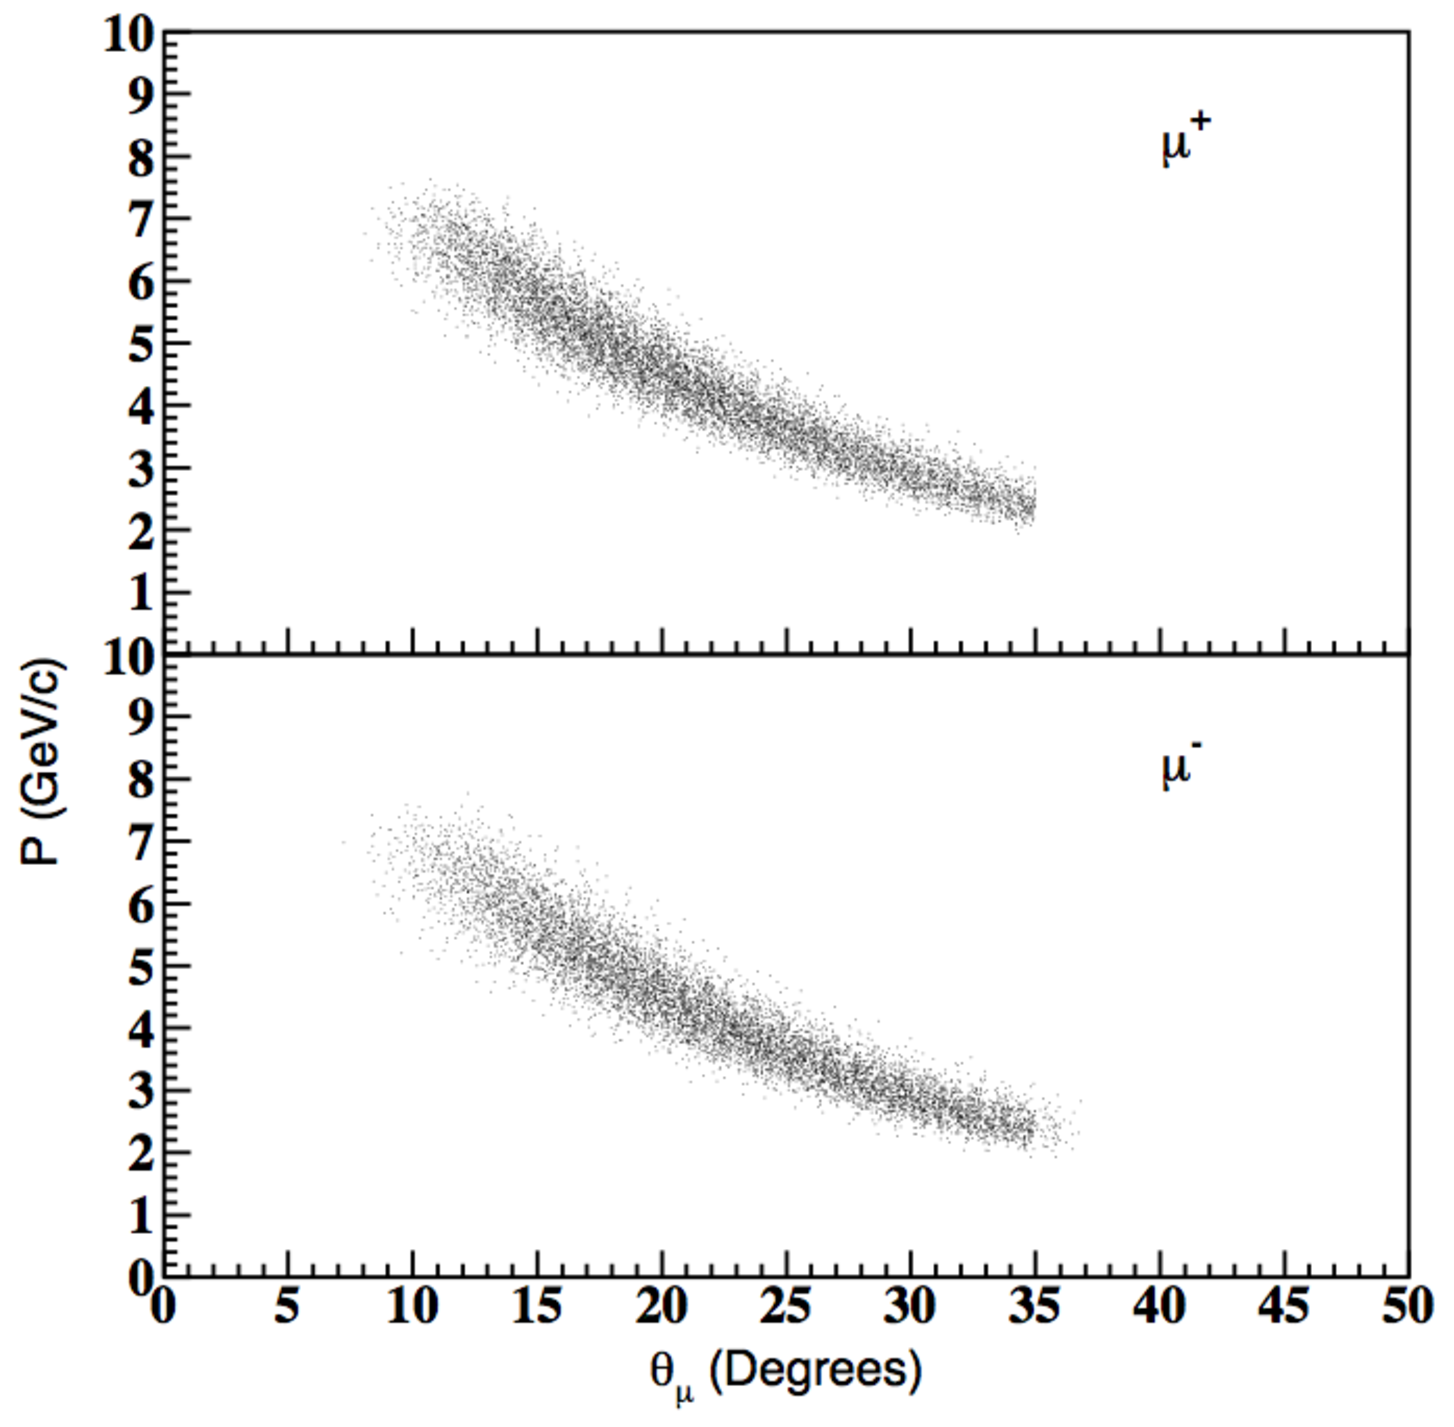
\includegraphics[width=0.6\textwidth]{jpsi_muon_p_theta_detected.pdf}
\caption{Angular-momentum distributions of $\mu^+$ (top) and $\mu^-$ bottom detected in the CLAS12 FD. }
\label{fig:jp_mukine}
\end{center}
\end{figure}

Since the proton will not be detected, when exclusivity is required the missing momentum analysis  of the $e\mu^+\mu^-$ final state will be performed to select events in the reaction $ep\to e^\prime p^\prime J/\Psi$, after identifying the $J/\Psi$ in the invariant mass of the muon pairs. For this, the mass (invariant and missing) resolution  will play an important role in identification of the reaction.  In Fig.\ref{fig:jp_mres} the expected resolutions for invariant and missing masses are shown. These distributions have been calculated using reconstructed, smeared, 3-momenta of the electron, $\mu^+$ and $\mu^-$ using the angular and momentum resolutions described above. Both distributions are fitted with Gaussian function. The standard deviations (mass resolutions) for both are $\sim 47$ MeV, indicating that identification of the J/$\Psi$ or the missing recoil proton is sufficient. 

\begin{figure}[htbp]
\begin{center}
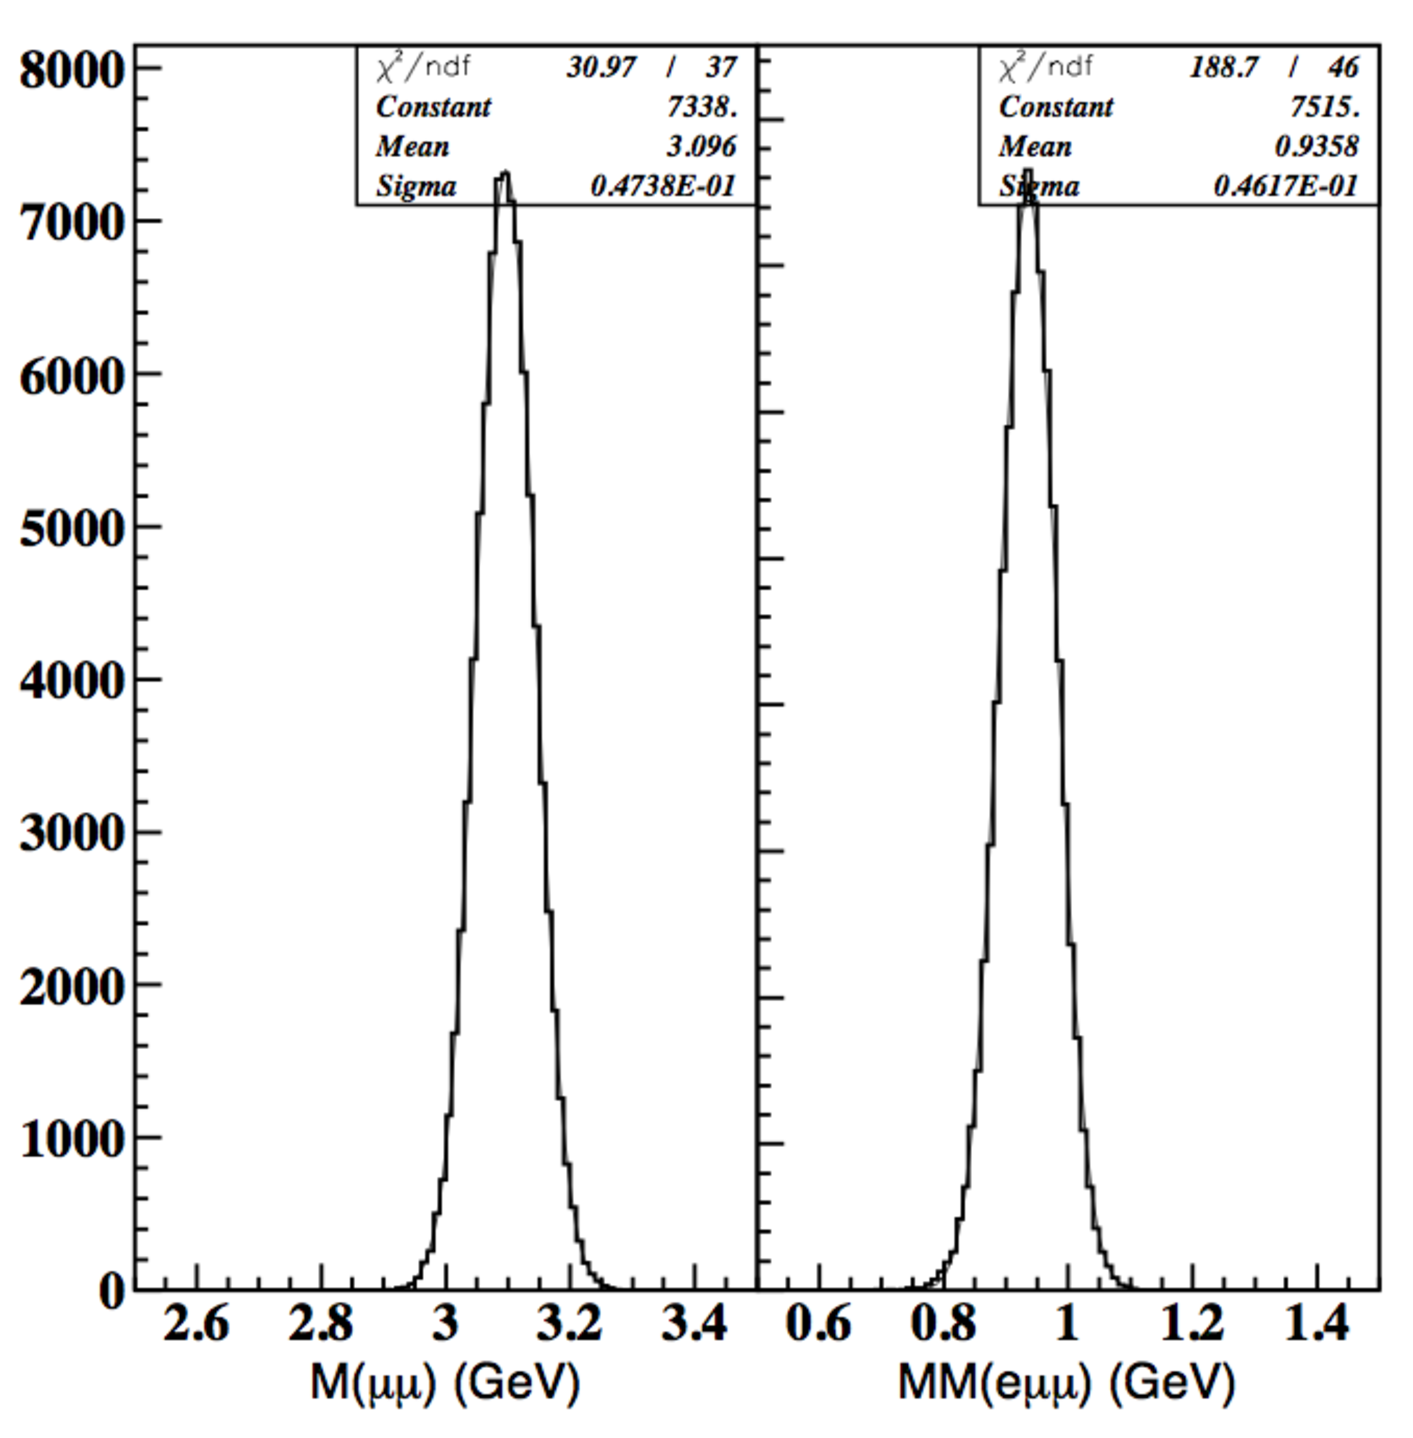
\includegraphics[width=.5\textwidth]{jpsi_minv_mmis_resolutions.pdf}
\caption{Expected mass resolutions: left the invariant mass of muon pairs, right the missing mass squared for the reaction $ep\to e^\prime \mu^+ \mu^- (p)$.}
\label{fig:jp_mres}
\end{center}
\end{figure}

As will be described below, the goal of the J/$\Psi$ electroproduction study will be the measurements of the t-dependence of the cross section in three bins of Q$^2$, $0.1<$Q$^2 <0.3$ GeV$^2$, $0.3<$Q$^2 <1.$ GeV$^2$, and $1<$Q$^2 < 2.5$ GeV$^2$. Therefore, our studies of the acceptances are also in these three bins of Q$^2$. The t-dependence of acceptances shown in Fig.\ref{fig:jp_acc}. The average acceptance for detection of (e$\mu^+\mu^-$) is about $\sim 3\%$, somewhat lower for lowest Q$^2$ bin. These acceptance values are used to calculate expected  rates. 

\begin{figure}[htbp]
\begin{center}
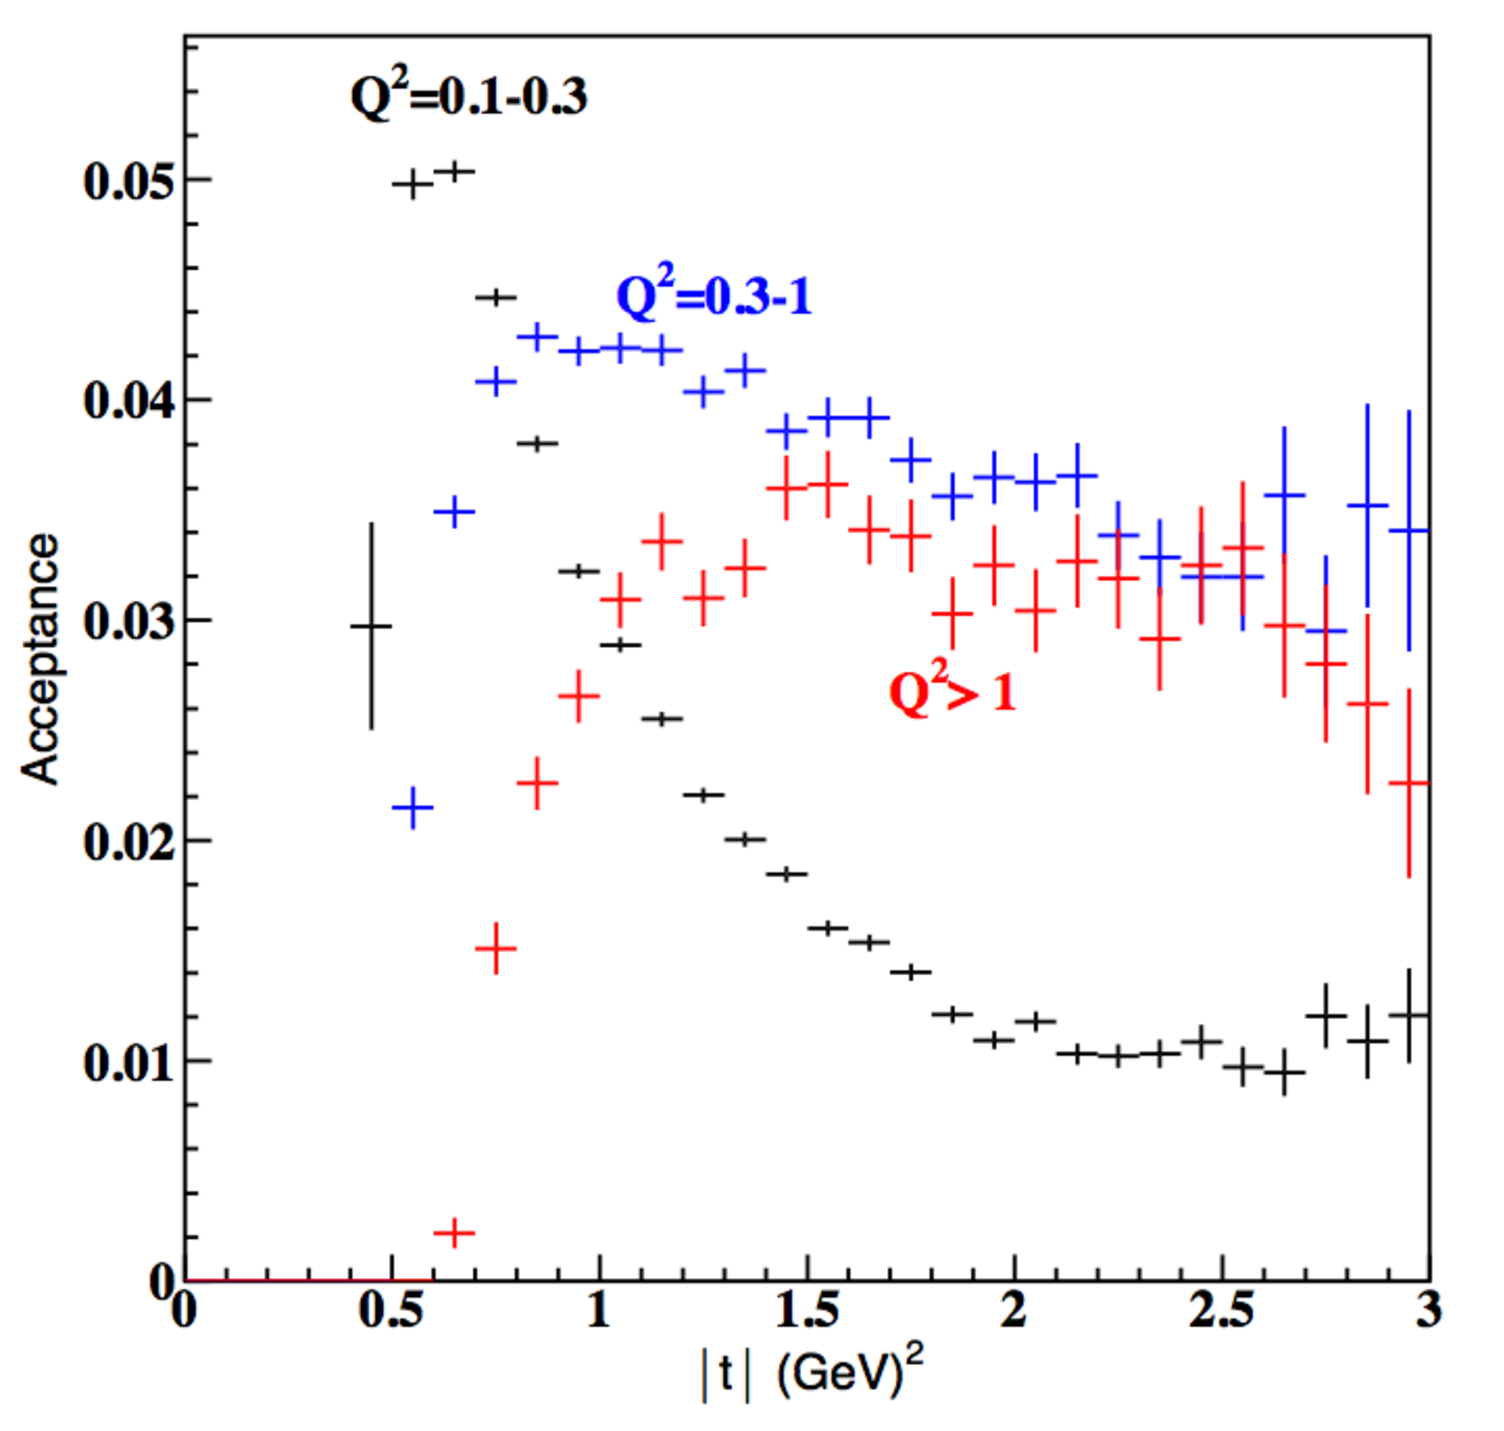
\includegraphics[width=.65\textwidth]{jpsi_t_acceptance_3Q2.pdf}
\caption{Acceptances as a function of $t$ for three Q$^2$ bins.}
\label{fig:jp_acc}
\end{center}
\end{figure}




%\clearpage